\documentclass[]{beamer}
%\documentclass[notes]{beamer}       % print frame + notes
%\documentclass[notes=only]{beamer}   % only notes
%\documentclass{beamer}              % only frames
%\documentclass[handout]{beamer}
\usepackage{tikz}
\usetikzlibrary{shapes.arrows,chains}

\usepackage{algorithm2e}

\usetheme{Dresden}%%%%% developer's preference - may change based on preferences

%%%%%% UMass official color: https://www.umass.edu/brand/elements/color
\definecolor{UMassAmherst}{rgb}{0.533 0.11 0.11}
\usecolortheme[named=UMassAmherst]{structure}

\title{Greedy y Programaci\'on din\'amica}
\author{MSc Edson Ticona Zegarra}
\institute{Campamento de Programaci\'on}
\date{}

%%%%%% obtained from: https://www.umass.edu/brand/elements/wordmarks-seal-and-spirit-marks
%%%%%% logos of other departments can also be obtained from the above link. Otherwise, consult your department website.

\begin{document}

\maketitle

\begin{frame}{Contenido}
\tableofcontents
\end{frame}

\section{Optimizaci\'on}
\begin{frame}{Contenido}
\tableofcontents[currentsection]
\end{frame}

\begin{frame}{Optimizaci\'on}
  \begin{definition}
    Un problema de optimizaci\'on es aquel en el que se busca la mejor soluci\'on dentro de un conjunto de soluciones v\'alidas
  \end{definition}
  \begin{itemize}
    \item Un problema de optimizaci\'on usualmente pide \textit{maximizar} o \textit{minimizar} alg\'un valor objetivo.
    \pause
    \item Por ejemplo, dado un conjunto de rutas posibles entre dos ciudades, hallar la ruta que minimice el tiempo de viaje.
    \pause
    \item En el ejemplo anterior, hay que notar que pueden existir m\'ultiples rutas que v\'alidas, pero no todas son \'optimas.
    \pause
    \item As\'i mismo, puede existir m\'as de una ruta \'optima, por tanto, m\'as de una soluci\'on \'optima. Estamos interesados en cualquier soluci\'on \'optima.
  \end{itemize}
\end{frame}

\section{Algoritmos greedy}
\begin{frame}{Contenido}
\tableofcontents[currentsection]
\end{frame}

\begin{frame}{Algoritmos \textit{Greedy}: voraces o golosos}
  \begin{itemize}
    \item Se llama algoritmo voraz a aquel que escoge la mejor opci\'on disponible en el momento.
      \pause
    \item Este tipo de algoritmos no observan opciones generales, sino que son muy focalizados en el momento.
      \pause
    \item Usualmente son eficientes y procesan un dato a la vez.
      \pause
    \item \textbf{No} todo problema de optimizaci\'on puede resuelto aplicando un algoritmo voraz.
      \pause
    \item Dado un problema, se debe demostrar que un algoritmo voraz encuentra una soluci\'on \'optima.
  \end{itemize}
\end{frame}

\section{Problemas}
\begin{frame}{Contenido}
\tableofcontents[currentsection]
\end{frame}

\subsection{Interval scheduling}
\begin{frame}{Interval scheduling}
  \begin{itemize}
    \item Dado un conjunto de intervalos que definen peticiones, se requiere atender el conjunto m\'aximo de intervalos de mayor tama\~no, dado que los intervalos no se sobrepongan.
      \pause
    \item Formalizando, sean $n$ intervalos, tal que el tiempo de inicio del intervalo $i$-\'esimo es $s(i)$ y el tiempo de finalizaci\'on es $f(i)$. Sea $S$ una soluci\'on, entonces $ \forall j, k \in S$, vale que $f(j)\leq s(k)$ o $f(k)\leq s(j)$. Una soluci\'on \'optima es aquella que maximiza $|S|$
  \end{itemize}
\end{frame}

\begin{frame}{Interval scheduling}
  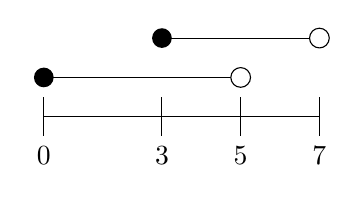
\begin{tikzpicture}[scale=0.5]
    \draw (0,0)-- (7,0); %Axis
    \foreach \x in {0,3,5,7} {
      \draw (\x,0.5) -- (\x,-0.5) node[below] {\x};
    }
    \draw (0,1) -- (5,1);
    \fill (0,1) circle (0.25);
    \draw[fill=white] (5,1) circle (0.25);
    %
    \draw (3,2) -- (7,2);
    \fill (3,2) circle (0.25);
    \draw[fill=white] (7,2) circle (0.25);
  \end{tikzpicture}
\end{frame}

\begin{frame}{Interval scheduling}
  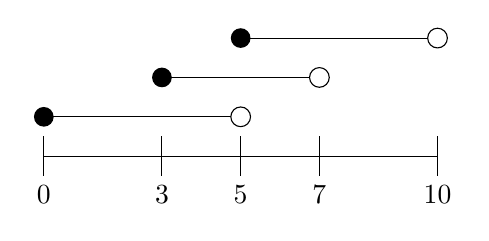
\begin{tikzpicture}[scale=0.5]
    \draw (0,0)-- (10,0); %Axis
    \foreach \x in {0,3,5,7,10} {
      \draw (\x,0.5) -- (\x,-0.5) node[below] {\x};
    }
    \draw (0,1) -- (5,1);
    \fill (0,1) circle (0.25);
    \draw[fill=white] (5,1) circle (0.25);
    %
    \draw (3,2) -- (7,2);
    \fill (3,2) circle (0.25);
    \draw[fill=white] (7,2) circle (0.25);
    %
    \draw (5,3) -- (10,3);
    \fill (5,3) circle (0.25);
    \draw[fill=white] (10,3) circle (0.25);
  \end{tikzpicture}
\end{frame}

\begin{frame}{Interval scheduling}
  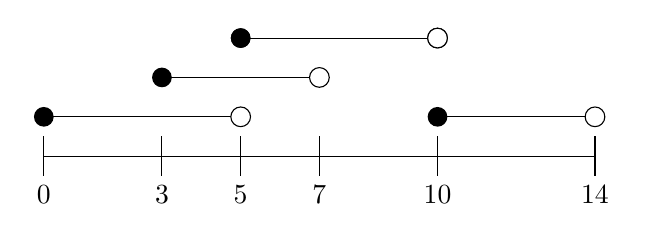
\begin{tikzpicture}[scale=0.5]
    \draw (0,0)-- (14,0); %Axis
    \foreach \x in {0,3,5,7,10,14} {
      \draw (\x,0.5) -- (\x,-0.5) node[below] {\x};
    }
    \draw (0,1) -- (5,1);
    \fill (0,1) circle (0.25);
    \draw[fill=white] (5,1) circle (0.25);
    %
    \draw (3,2) -- (7,2);
    \fill (3,2) circle (0.25);
    \draw[fill=white] (7,2) circle (0.25);
    %
    \draw (5,3) -- (10,3);
    \fill (5,3) circle (0.25);
    \draw[fill=white] (10,3) circle (0.25);
    %
    \draw (5,3) -- (10,3);
    \fill (5,3) circle (0.25);
    \draw[fill=white] (10,3) circle (0.25);
    %
    \draw (10,1) -- (14,1);
    \fill (10,1) circle (0.25);
    \draw[fill=white] (14,1) circle (0.25);
  \end{tikzpicture}
\end{frame}

\begin{frame}{Algoritmo voraz}
  \begin{enumerate}
    \item Seleccionar, bajo alguna estrategia, un intervalo $i$
    \item Eliminar todos aquellos intervalos no compatibles con el intervalo $i$
    \item Repetir hasta que todos los intervalos sean procesados
  \end{enumerate}
  \pause
  \begin{itemize}
    \item Usualmente esta estructura b\'asica se repite en varios problemas que admiten soluciones greedy
      \pause
    \item ?`Qu\'e estrategia se debe usar para seleccionar un intervalo?
  \end{itemize}
\end{frame}

\begin{frame}{Soluci\'on}
  \begin{itemize}
    \item Seleccionar aquel intervalo que tenga el menor tiempo de finalizaci\'on
  \end{itemize}
  \begin{algorithm}[H]
    \SetKwInOut{Input}{input}\SetKwInOut{Output}{output}
    \Input{$I=(s,f)$ es el conjunto de $n$ intervalos}
    \Output{$S$ conjunto m\'aximo de intervalos}
    \BlankLine
    $Sort(I)\ por\ f$ \;
    $S \leftarrow \{I[0]\}$ \;
    $time \leftarrow I[0].f$\;
    \For{$i \in I\setminus \{I[0]\}$}
    {
      \If{$time \leq i.s$}
      {
        $S.append(i)$ \;
        $time \leftarrow i.f$
      }
    }
    \KwRet{$S$}
  \end{algorithm}
\end{frame}

\subsection{Problema de la mochila fraccionaria}
\begin{frame}{Problema de la mochila fraccionaria}
  \begin{itemize}
    \item Dado un conjunto de elementos, cada uno con un valor $v$ y un peso $w$, y dada un mochila de capacidad $W$, se requiere llenar la mochila con la mayor cantidad de elementos tal que el valor total de los objetos sea m\'aximo sin sobrepasar la capacidad de la mochila. Note que los elementos pueden ser partidos en fracciones.
      \pause
    \item Formalizando, sean $n$ elementos $E=(v,w)$, se busca un subconjunto de elementos $S\subset E$ tal que $\sum_{s \in S} s.v $ es el m\'aximo posible y $\sum_{s \in S} s.w \leq W$
  \end{itemize}
\end{frame}

\begin{frame}{Soluci\'on}
  \begin{itemize}
    \item Seleccionar los elementos que tengan un mayor ratio $v_i/w_i$
  \end{itemize}
\end{frame}

\begin{frame}{Soluci\'on}
  \begin{algorithm}[H]
    \SetKwInOut{Input}{input}\SetKwInOut{Output}{output}
    \Input{$E=(v,w)$ es el conjunto de elementos y $W$ el tama\~no de la mochila}
    \Output{$S$ conjunto de elementos en la mochila}
    \BlankLine
    $Sort(E)\ por\ v/w$ \;
    $value \leftarrow 0$ \;
    $c \leftarrow W$ \tcc*{capacidad disponible en la mochila}
    \For{$e \in E$}
    {
      \If{$c < e.w$}
      {
        $value \leftarrow value + e.v/e.w*(W-c)$ \;
        $break$
      }
      $value \leftarrow value + e.v$ \;
      $c \leftarrow c-e.w$ \;
    }
    \KwRet{$value$}
  \end{algorithm}
\end{frame}

\section{Programaci\'on Din\'amica}
\begin{frame}{Contenido}
\tableofcontents[currentsection]
\end{frame}

\begin{frame}{Dynamic Programming (DP)}
  \begin{itemize}
    \item Es una t\'ecnica de dise\~no de algoritmos usualmente utilizada para resolver problemas de optimizaci\'on
      \pause
    \item De manera an\'aloga a la t\'ecnica de divide y vencer\'as, DP tambi\'en divide el problema en subproblemas
      \pause
    \item La diferencia es que los subproblemas se sobreponen, y la soluci\'on a cada subproblema es guardada en una tabla
      \pause
    \item Usualmente la complejidad es, al menos, cuadr\'atica
  \end{itemize}
\end{frame}

\begin{frame}{Dynamic Programming (DP)}
  \begin{itemize}
    \item DP es utilizado para resolver problemas de optimizaci\'on que satisfacen el \textit{principio de optimalidad}: en una secuencia de decisiones \'optimas, cada subsecuencia debe ser tambi\'en \'optima
      \pause
    \item Esto puede parecer obvio pero no siempre aplica
      \pause
    \item Alternativamente se puede definir para los problemas que aplica el principio de optimalidad: la soluci\'on \'optima a cualquier instancia no trivial es una combinaci\'on de soluciones \'optimas de algunas de sus subinstancias. 
  \end{itemize}
\end{frame}

\begin{frame}{Dynamic Programming (DP)}
  \begin{itemize}
    \item Primero se debe caracterizar la estructura de una soluci\'on \'optima
      \pause
    \item Luego, se define recursivamente el valor de una soluci\'on \'optima
      \pause
    \item Computar el valor de la soluci\'on \'optima, usualmente de ``arriba hacia abajo'' (recursi\'on y memorizaci\'on)
      \pause
    \item Construir la soluci\'on \'optima de la informaci\'on hallada
  \end{itemize}
\end{frame}

\section{Problemas}
\begin{frame}{Contenido}
\tableofcontents[currentsection]
\end{frame}

\subsection{Mayor secuencia palindr\'omica}
\begin{frame}{Mayor secuencia palindr\'omica}
  \begin{definition}
    Un pal\'indrome es una secuencia de caracteres que se lee igual de izquierda a derecha como de derecha a izquierda.
    Por ejemplo: ``radar'', ``221122'', ``oso'', ``aerea'', ``ala''
  \end{definition}
  \begin{itemize}
    \item En el problema es dada una secuencia de caracteres y se busca la subsecuencia m\'as larga tal que sea un pal\'indromo
      \pause
    \item Por ejemplo, dado ``character'', las subsecuencias palindr\'omicas son ``t'', ``ara'', ``carac''. La mayor de ellas es ``carac''
  \end{itemize}
\end{frame}

\begin{frame}{Mayor secuencia palindr\'omica}
  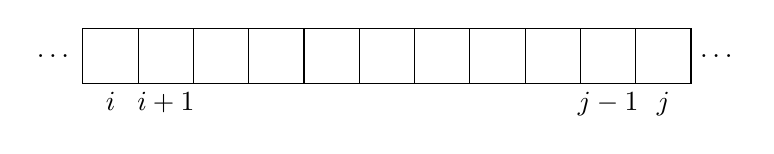
\begin{tikzpicture}[
      start chain=1 going right,start chain=2 going right,node distance=-0.15mm
    ]
    \node [on chain=1] at (-1.5,-.4) {\ldots};  
    \foreach \x in {1,2,...,11} {
      \x, \node [draw,on chain=1,minimum size=2em] (n\x) {};
    } 
    \node [name=r,on chain=1] {\ldots}; 
    \node[below=of n1]  {$i$};
    \node[below=of n2]  {$i+1$};
    \node[below=of n11] {$j$};
    \node[below=of n10] {$j-1$};
  \end{tikzpicture}
  \pause
  \begin{itemize}
    \item $L(i,j) = \max \{L(i,j-1), L(i+1,j)\}$
      \pause
    \item Trivialmente, cualquier secuencia de tama\~no 1 es un pal\'indromo, siendo este el caso base
  \end{itemize}
\end{frame}

\begin{frame}{LCP}
  \begin{algorithm}[H]
    \SetKwInOut{Input}{input}\SetKwInOut{Output}{output}
    \Input{$S$ es la secuencia de caracteres en $i$ y $j$ indican los l\'imites}
    \Output{$l$ longitud de la mayor secuencia palindr\'omica}
    \BlankLine
    \If{$i == j$}
    {
      \KwRet{1}
    }
    \If{$S[i] == S[j]$}
    {
      \KwRet{$ 2 + LCP(i+1,j-1) $}
    } \Else {
      \KwRet{$\max \{ LCP(i,j-1), LCP(i+1,j) \} $}
    }
  \end{algorithm}
\end{frame}

\begin{frame}{Complejidad}
  \begin{itemize}
    \item $T(n) = 2T(n-1) = 2^{n-1}$ 
      \pause
    \item Hay $\binom{n}{2}$ subproblemas distintos, uno para cada par $(i,j)$ tal que $i<j$. 
      \pause
    \item Resolviendo cada problema una sola vez, $\Theta(n^2) \times \theta(1) = \Theta(n^2)$, dado que cada subproblema tenga los sub-subproblemas resueltos.
  \end{itemize}
\end{frame}

\begin{frame}{Memorizaci\'on vs Iteraci\'on}
  \begin{itemize}
    \item En general, memorizaci\'on utiliza un diccionario (map) donde para cada para $i,j$ se almacena el valor de $L$. En particular, para este ejemplo basta con un arreglo bidimensional.
      \pause
    \item La otra alternativa es resolver iterativamente, desde los problemas m\'as peque\~nos a los m\'as grandes.
      \pause
    \item Teniendo la misma complejidad temporal pero diferente complejidad espacial.
      \pause
    \item En algunos casos, se puede mejorar la cantidad de memoria necesaria manteniendo \'unicamente las partes necesarias de la matriz
  \end{itemize}
\end{frame}

%\begin{frame}{Mayor secuencia palindr\'omica}
%  \begin{definition}
%    Un pal\'indrome es una secuencia de caracteres que se lee igual de izquierda a derecha como de derecha a izquierda.
%    Por ejemplo: ``radar'', ``221122'', ``oso'', ``aerea'', ``ala''
%  \end{definition}
%  \begin{itemize}
%    \item En el problema es dada una secuencia de caracteres y se busca la subsecuencia m\'as larga tal que sea un pal\'indromo
%      \pause
%    \item Por ejemplo, dado ``character'', las subsecuencias palindr\'omicas son ``t'', ``ara'', ``carac''. La mayor de ellas es ``carac''
%  \end{itemize}
%\end{frame}

\subsection{Juego de la moneda}
\begin{frame}{Juego de la moneda}
  \begin{itemize}
    \item Dadas $n$ monedas con valores $v_1, v_2, ..., v_n$, siendo $n$ par; se tiene un juego por turnos para 2 personas
      \pause
    \item En cada turno, el jugador toma la primera o la \'ultima moneda, recibiendo el valor de dicha moneda
      \pause
    \item Gana el jugador que obtiene un valor mayor
      \pause
    \item ?`El jugador que inicia la partida podr\'a ganar siempre?
  \end{itemize}
\end{frame}

\begin{frame}{Juego de la moneda: ejemplos}
  \begin{itemize}
    \item $4, 42, 39, 17, 25, 6$
      \pause
    \item $8, 15, 3, 7$
      \pause
    \item ?`Una estrategia greedy funciona?
  \end{itemize}
\end{frame}

\begin{frame}{Juego de la moneda}
  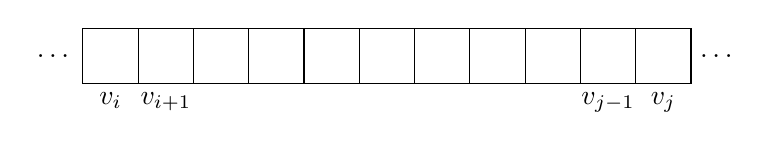
\begin{tikzpicture}[
      start chain=1 going right,start chain=2 going right,node distance=-0.15mm
    ]
    \node [on chain=1] at (-1.5,-.4) {\ldots};  
    \foreach \x in {1,2,...,11} {
      \x, \node [draw,on chain=1,minimum size=2em] (n\x) {};
    } 
    \node [name=r,on chain=1] {\ldots}; 
    \node[below=of n1]  {$v_i$};
    \node[below=of n2]  {$v_{i+1}$};
    \node[below=of n11] {$v_j$};
    \node[below=of n10] {$v_{j-1}$};
  \end{tikzpicture}
  \begin{itemize}
    \item Sea $V(i,j)$ el valor m\'aximo que podemos ganar en nuestro turno cuando quedan las monedas $v_i$ hasta $v_j$
      \pause
    \item Entonces, $V(i,j)$ tiene dos opciones: o seleccionamos $v_i$ o seleccionamos $v_j$
  \end{itemize}
\end{frame}

\begin{frame}{Juego de la moneda}
  \begin{itemize}
    \item El oponente tratar\'a de hacer la mejor jugada posible
      \pause
    \item Por ello, luego de nosotros haber seleccionado una moneda, el oponente nos dejar\'a con el menor valor posible de las monedas que quedan
      \pause
    \item Entonces, si nosotros seleccionamos $v_i$, el oponente seleccionar\'a tal que lo que nos quede sea el m\'inimo entre $(v_{i+2}, v_j)$ y $(v_{i+1}, v_{j-1})$
      \pause
    \item Analogamente, si nosotros seleccionamos $v_j$, el oponente seleccionar\'a tal que lo que nos quede sea el m\'inimo entre $(v_{i}, v_{j-2})$ y $(v_{i+1}, v_{j-1})$
  \end{itemize}
\end{frame}

\begin{frame}{Complejidad}
  \begin{itemize}
    \item $V(i,j) = \max \biggl\{ v_i + \min \{V(i+1,j-1), V(i+2,j) \} , v_j + \min \{ V(i, j-2), V(i+1, j-1) \} \biggl\} $
      \pause
    \item Hay $\binom{n}{2}$ subproblemas distintos
      \pause
    \item Resolviendo cada problema una sola vez, $\Theta(n^2) \times \theta(1) = \Theta(n^2)$, dado que cadasubproblema tenga los sub-subproblemas resueltos.
  \end{itemize}
\end{frame}

\begin{frame}{Jugada}
  \begin{algorithm}[H]
    \SetKwInOut{Input}{input}\SetKwInOut{Output}{output}
    \Input{$V$ los valores de las $n$ monedas, $i$ y $j$ los l\'imites}
    \Output{Secuencia de monedas a elegir}
    \BlankLine
    \If{$i == j$}
    {
      \KwRet{$V[i]$}
    }
    $jugada1 \leftarrow \min (Jugada(i+2, j) , Jugada(i+1, j-1)) + V[i]$ \;
    $jugada2 \leftarrow \min (Jugada(i+1, j-1) , Jugada(i, j-2)) + V[j]$ \;
    \KwRet{$\max \{ jugada1, jugada2 \} $}
  \end{algorithm}
\end{frame}

\begin{frame}{Top-down vs Bottom-up}
  \begin{itemize}
    \item Ambas versiones son equivalentes, es decir, ambas solucionan el problema correctamente
      \pause
    \item En t\'erminos de complejidad temporal, son equivalentes
      \pause
    \item Sin embargo, difieren en t\'erminos de complejidad espacial
      \pause
    \item Para que la soluci\'on sea eficiente, la forma top-down usualmente necesita de memorizaci\'on
  \end{itemize}
\end{frame}


\end{document}
